
\documentclass[10pt]{beamer}

\usepackage[utf8]{inputenc}
\usepackage[ngerman]{babel}

\usetheme{metropolis}
\usepackage{appendixnumberbeamer}

\usepackage{booktabs}
\usepackage[scale=2]{ccicons}

\usepackage{verbatim}

\newcommand{\themename}{\textbf{\textsc{metropolis}}\xspace}

\title{API-Usability}
\subtitle{Effekte der Konstruktoren}
\date{21. August 2018}
\author{Elias Hofele, David Oberacker und Calvin Urankar}
\institute{Institut für Telematik, Telecooperation Office (TECO), Karlsruher Institut für Technologie}
\titlegraphic{\hfill
\includegraphics[height=0.5cm]{TECO_Logo.jpg}}

\begin{document}
    
    \maketitle
    
%    \begin{frame}{Table of contents}
%    \setbeamertemplate{section in toc}[sections numbered]
%    \tableofcontents[hideallsubsections]
%	\end{frame}

\section{Motivation}

	\begin{frame}[fragile]{APIs \& Benutzbarkeit}
		\metroset{block=fill}
		\begin{block}{Usability}
			\textit{Extent to which a system, product or service can be used by specified users to achieve specified goals with effectiveness,
				efficiency and satisfaction in a specified context of use.}	
			\hfill - ISO 9241-11
		\end{block}
		\vspace{\baselineskip}
		\begin{block}{API Usability i}
			\textit{[...] four main research questions, which characterize fundamental aspects of usability: understandability, abstraction level, reusability, and learnability.}	
			\hfill - Piccioni, Furia \& Meyer
		\end{block}
		\begin{block}{API Usability ii}
			\textit{The first-level arributes are: Knowability, Operability, Efficiency, Robustness, Safety, Subjective satisfaction.}	
			\hfill - Mosqueira-Rey, et. al
		\end{block}
	
	\end{frame}

	\begin{frame}[fragile]{Default vs. Required}
		\begin{columns}[T,onlytextwidth]
			
			\begin{column}{0.45\textwidth}
				\begin{center}\textit{create-set-call}\end{center}
				\begin{verbatim}
					var foo = new FooClass();
					foo.setBar(barValue);
					foo.use();
				\end{verbatim}
			\end{column}
			\vrule{}
			\begin{column}{0.02\textwidth}
			\end{column}
			\begin{column}{0.53\textwidth}
				\begin{center}\textit{create-call}\end{center}
				\begin{verbatim}
					var foo = new FooClass(barValue);
					foo.use();
				\end{verbatim}
			\end{column}
			
		\end{columns}
	\end{frame}

	\begin{frame}{Verwandte Arbeiten}
		\begin{quote}
			We found the create-set-call pattern to be more
			usable than, and preferred to, required constructors.
		\end{quote}
		\hfill - Stylos \& Clarke\\
		\vspace{\baselineskip}
		\vspace{\baselineskip}
		\begin{quote}
			In our study, however, the participants had no particular
			difficulties with using constructors with arguments [...]. 
		\end{quote}
		\hfill - Piccioni, Furia \& Meyer
	
	
	\end{frame}

\section{Forschungsfrage \& Hypothese}

	\begin{frame}[standout]{Hypothese}
		Semantische Fehler im Quellcode werden mit Default-Konstruktoren schneller entdeckt
		\begin{center}\small{und}\end{center}
		Konstruktoren haben keinen Einfluss auf das Finden von syntaktischen Fehlern.
	\end{frame}

	\begin{frame}{Nutzerstudie}
		\begin{itemize}
			\item Web-basierte Studie\\
			\vspace{\baselineskip}
			\item Vier Codeschnipsel pro Proband\\
			\vspace{\baselineskip}
			\item Fehlersuche\\
			\vspace{\baselineskip}
			\item Within subjects
		\end{itemize}
	\end{frame}

	\begin{frame}{Variablen}
		\begin{columns}[T,onlytextwidth]
	
			\column{0.5\textwidth}
			Abhängige Variablen
			\begin{itemize}
				\item Anzahl gefundener Fehler
				\item Zeit
				\item Lesefokus (Areas of Interest)
				\begin{itemize}
					\item Dokumentation
					\item Pre-Defekt
					\item Defekt
					\item Post-Defekt
				\end{itemize}
			\end{itemize}
		
			\column{0.5\textwidth}
			Unabhängige Variablen
			\begin{itemize}
				\item Art des Konstruktors:
				\begin{itemize}
					\item Default
					\item Required
				\end{itemize}
				\item Art des Fehlers:
				\begin{itemize}
					\item Syntaktisch
					\item Semantisch
				\end{itemize}
			\end{itemize}
		\end{columns}	
	\end{frame}

\section{Experimentalaufbau}

	\begin{frame}{Aufgabenkriterien}
		\begin{itemize}
			\item Plausibilität\\
			\vspace{\baselineskip}
			\item Komplexität\\
			\vspace{\baselineskip}
			\item Länge
			\begin{itemize}
				\item $\sim$ 100 Zeilen Dokumentation
				\item $\sim$ 80 Zeilen Code
			\end{itemize}
			\vspace{\baselineskip}
			\item Untereinander unabhängig (Minimierung der Lerneffekte)\\
		\end{itemize}
	\end{frame}

	\begin{frame}{Peter  i}
		\begin{figure}
			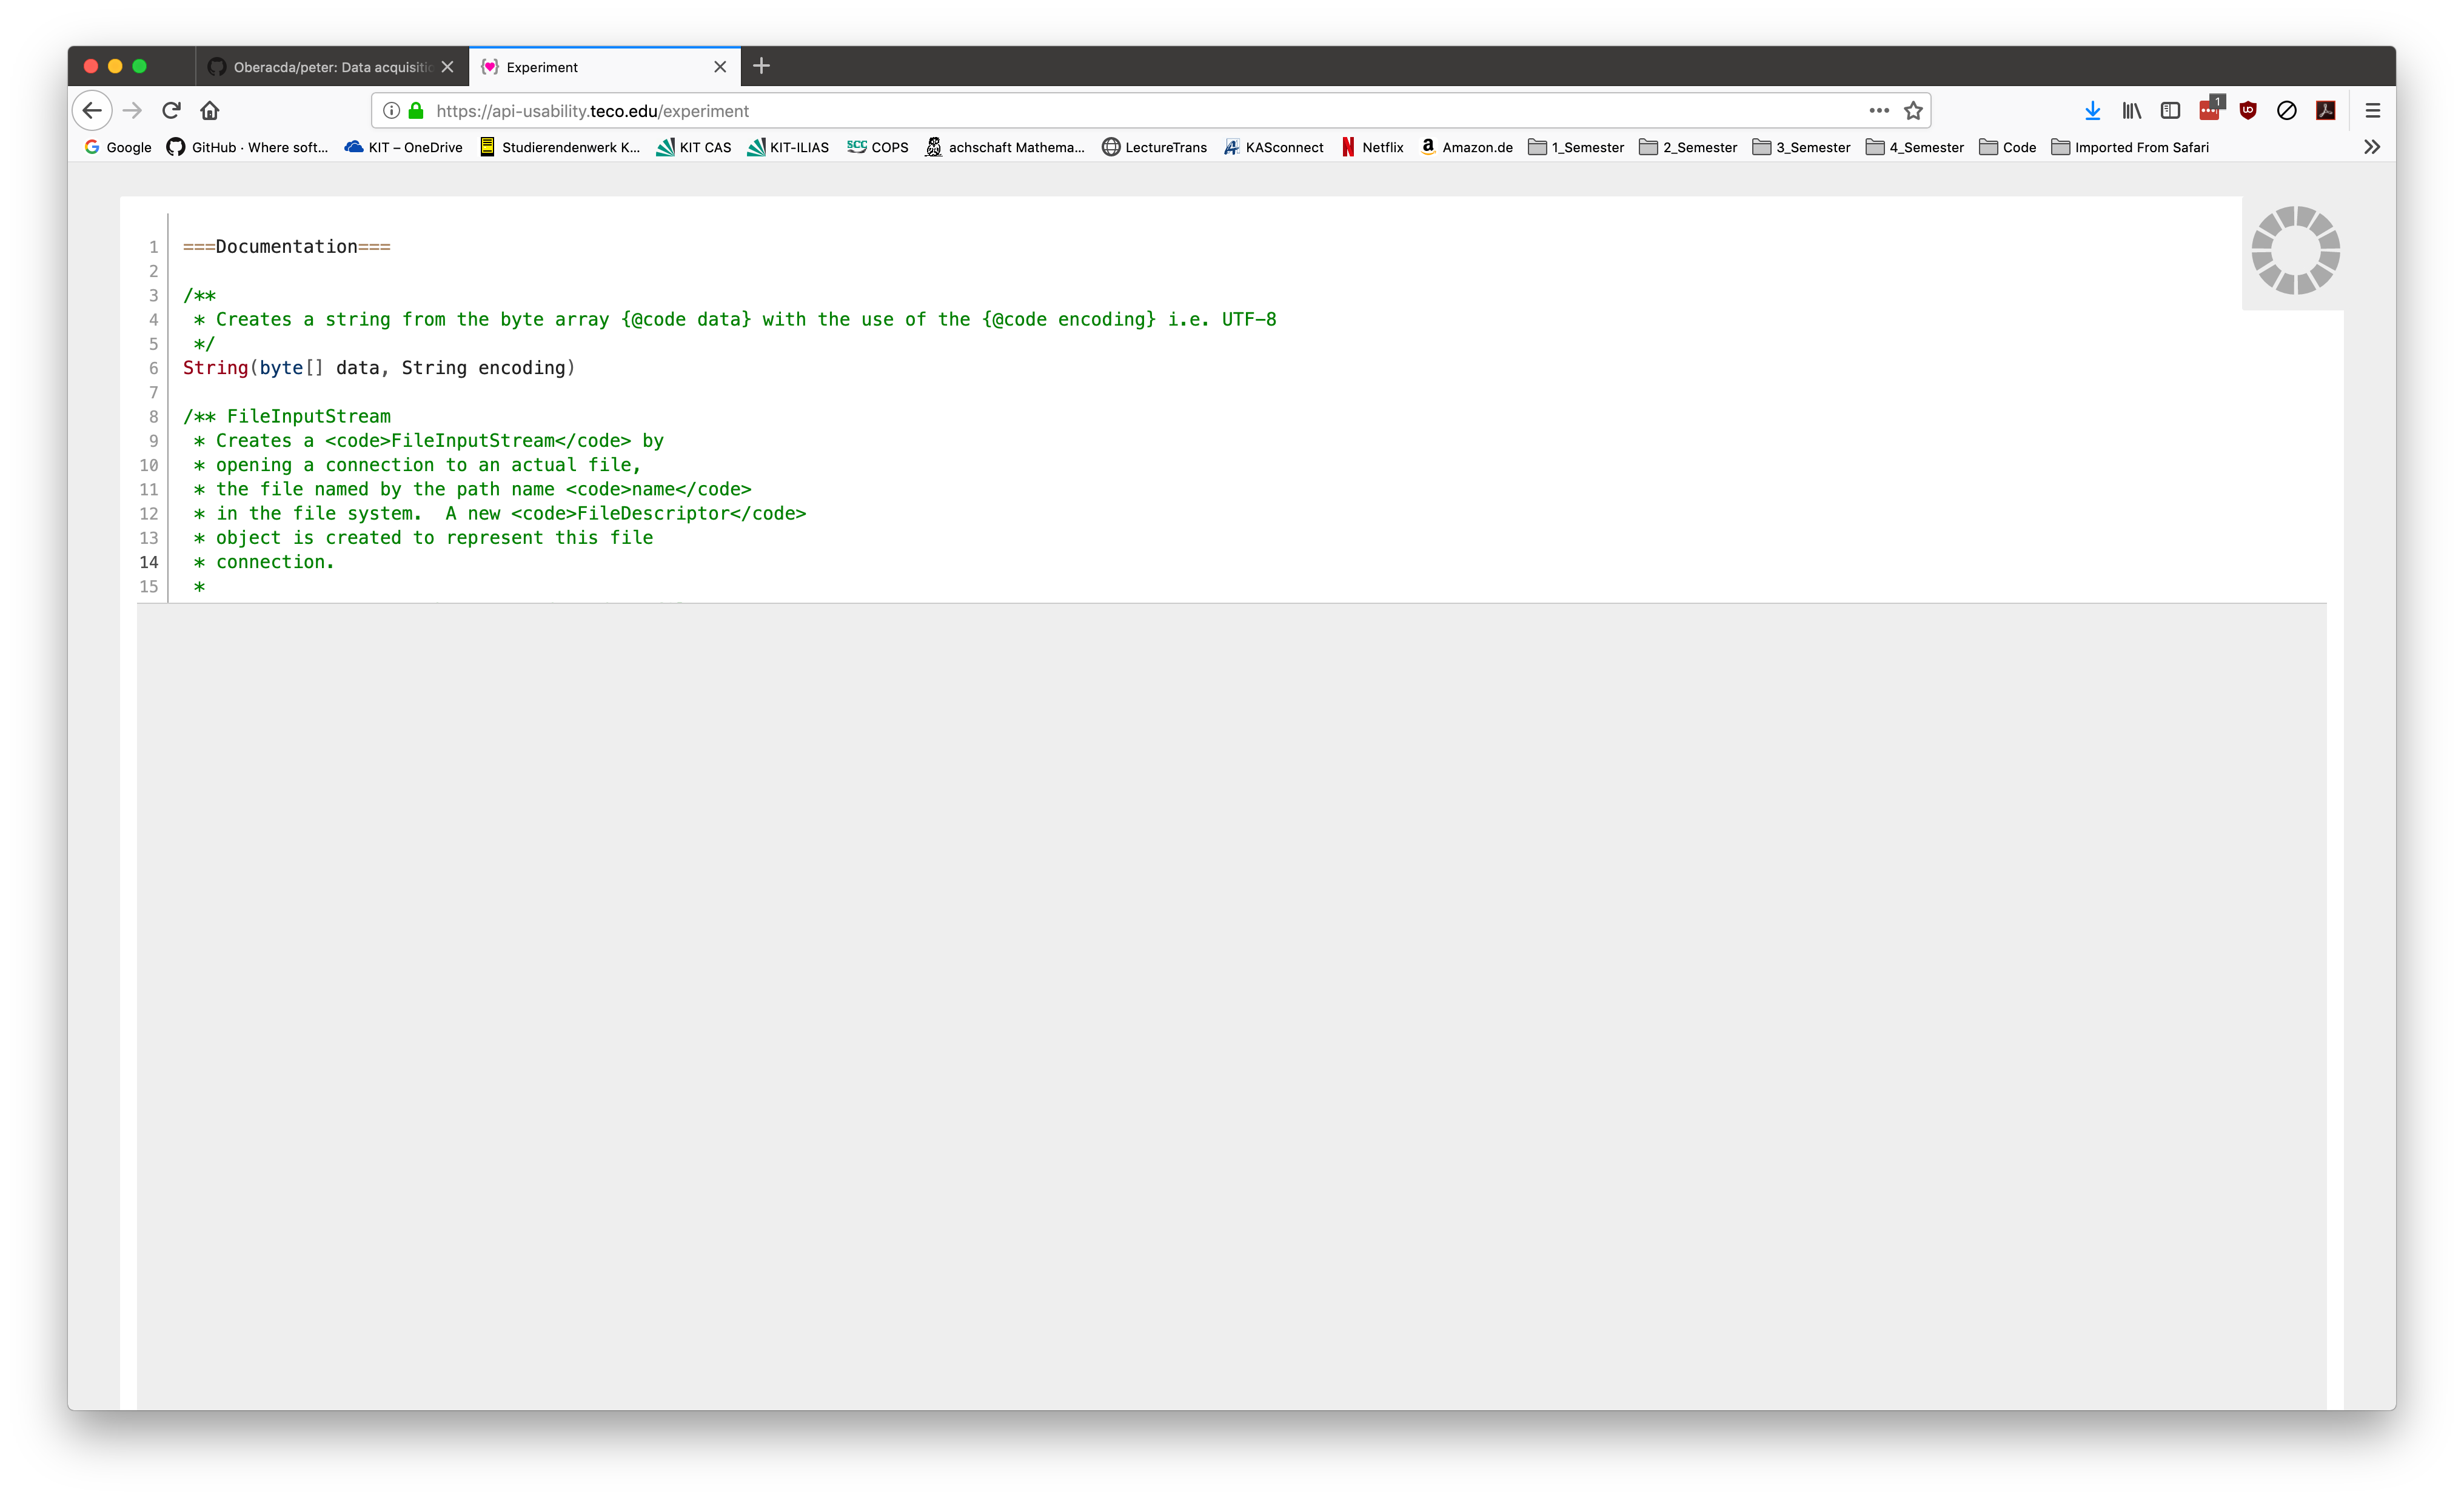
\includegraphics[scale=0.15]{graphics/peter_window.png}
			\caption{\label{fig:peter_window.png} Probanden sahen stets nur einen Ausschnitt des Quellcodes, welchen sie jedoch nach oben und unten bewegen konnten.}
		\end{figure}
	\end{frame}

	\begin{frame}{Peter  ii}	
		\begin{figure}
			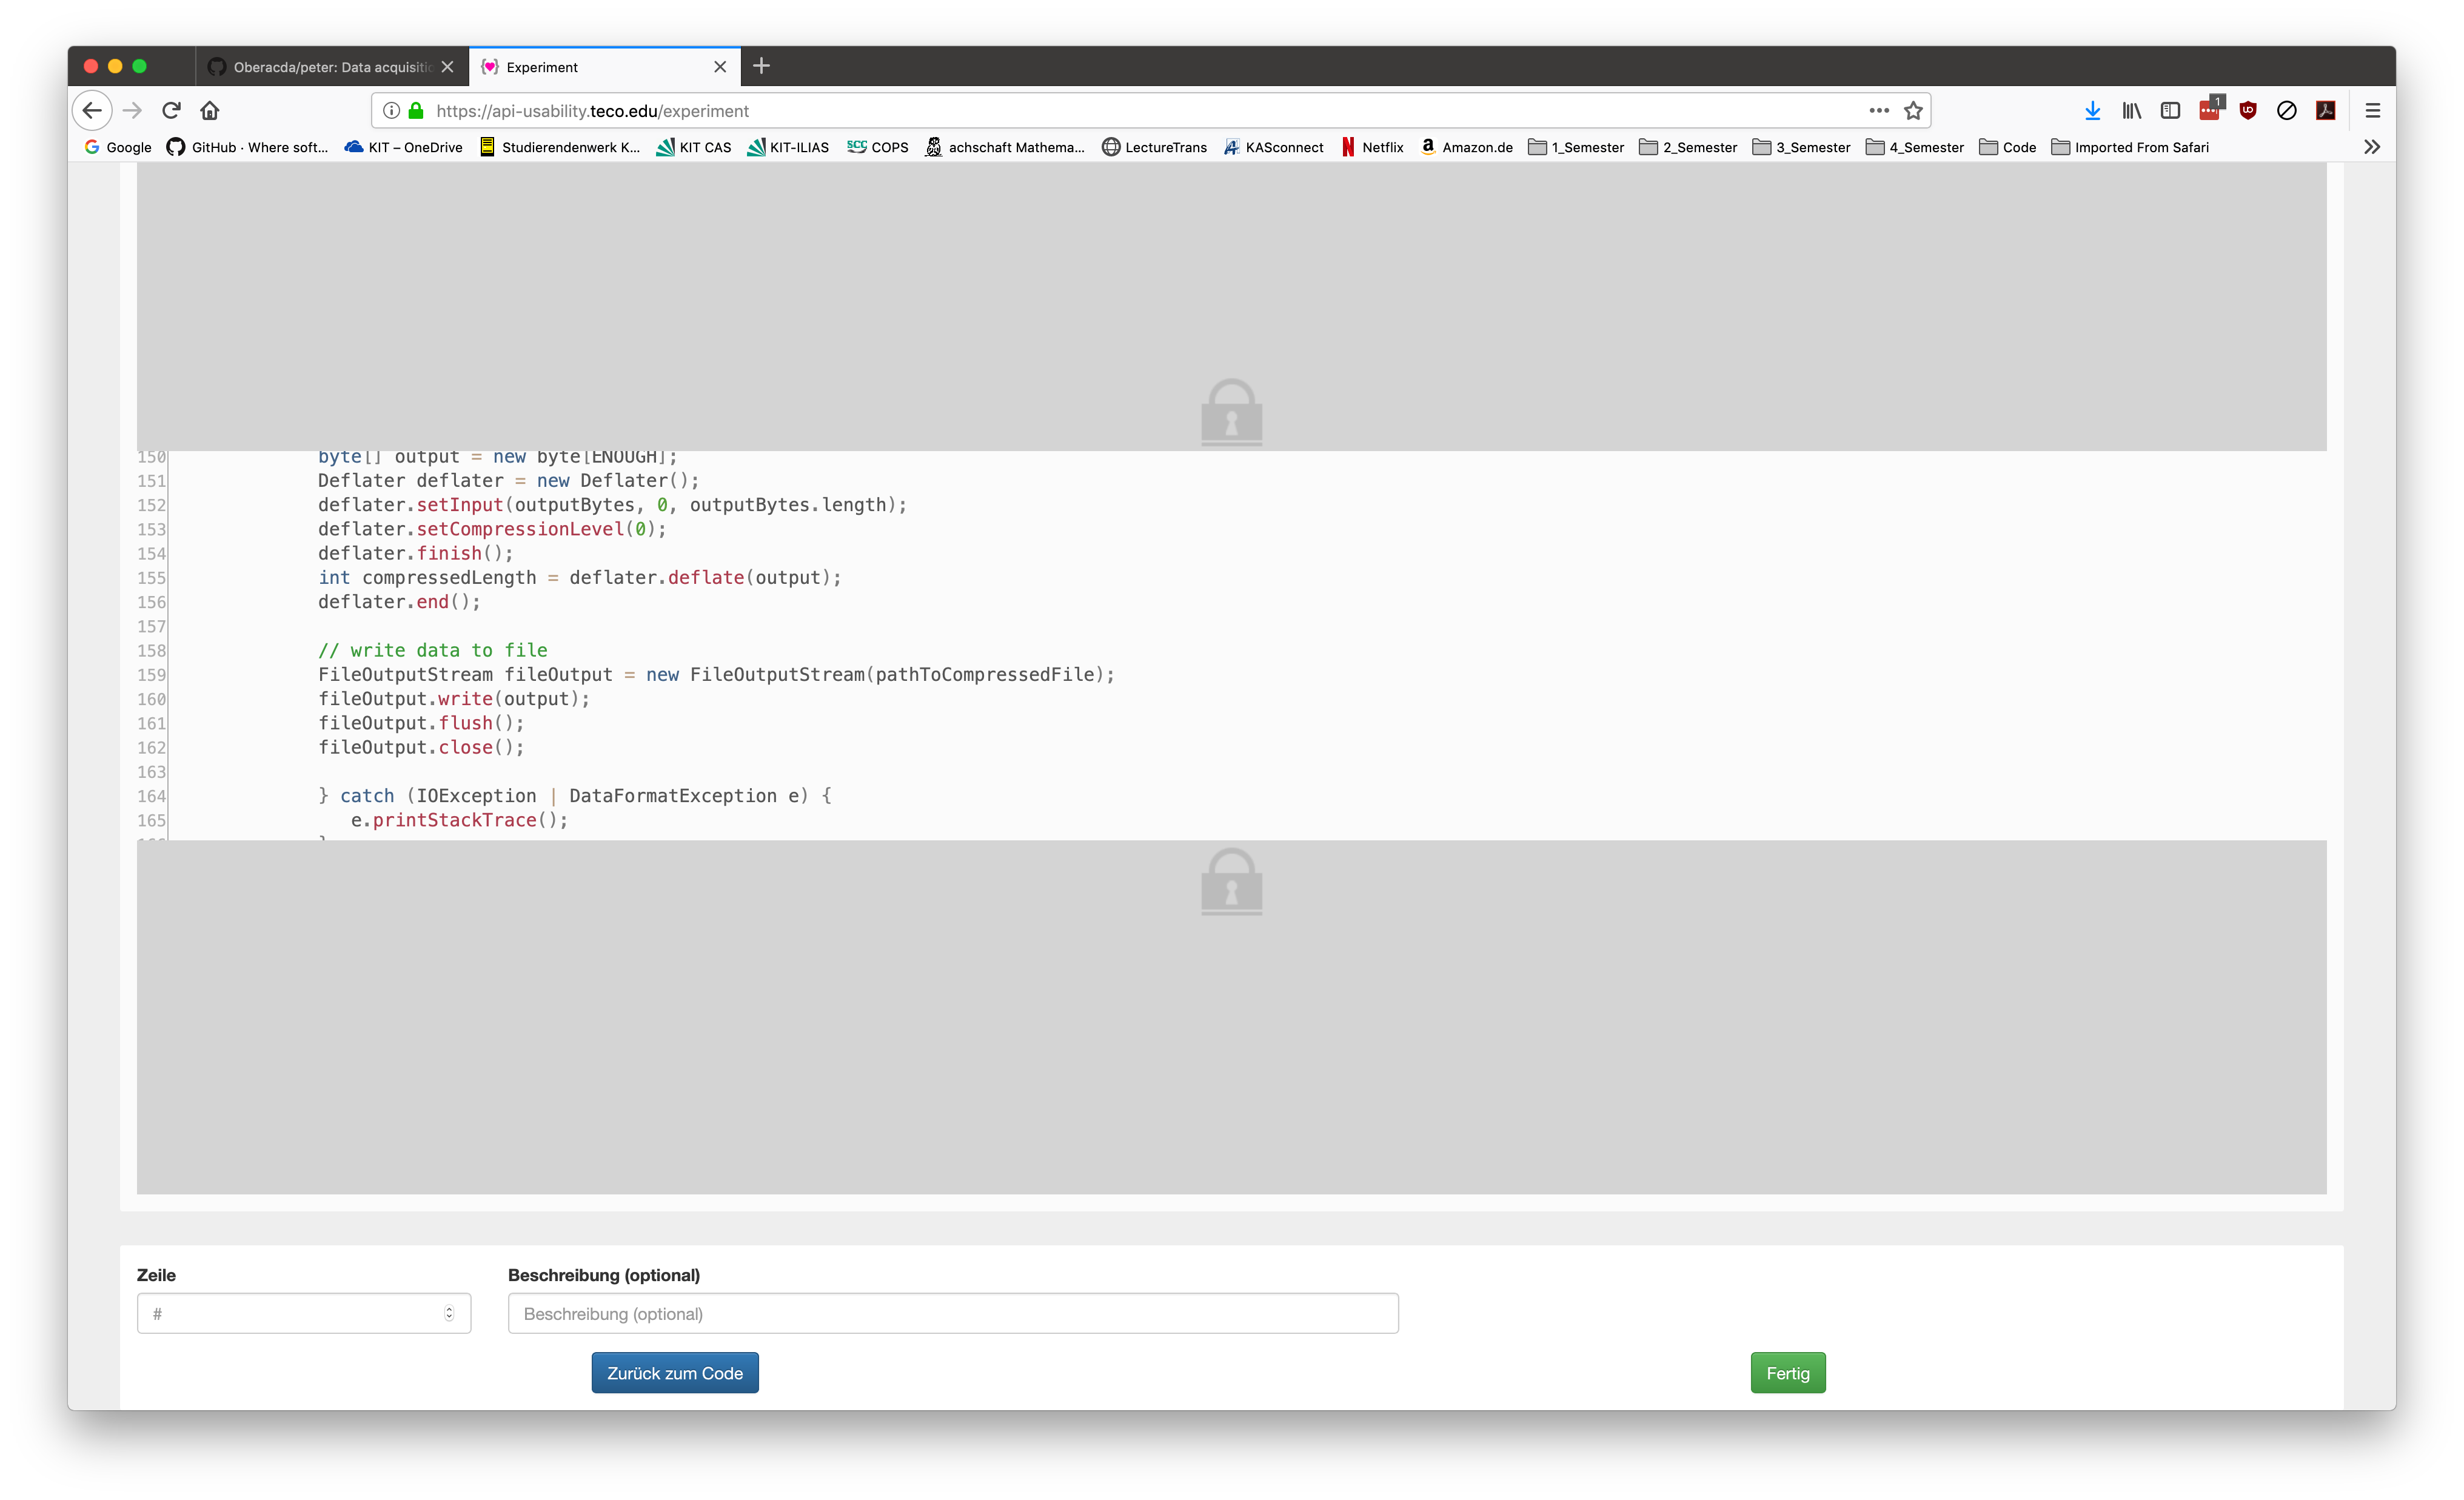
\includegraphics[scale=0.15]{graphics/peter_correction.png}
			\caption{\label{fig:peter_correction.png} Durch das Drücken der Leertaste konnten sie indizieren das sie den Fehler gefunden hatten.}
		\end{figure}
	\end{frame}

\section{Resultate}

	\begin{frame}{Stichprobenbeschreibung}
	 
	\end{frame}

	\begin{frame}{Bearbeitungszeit nach Konstruktor}
		\begin{figure}
			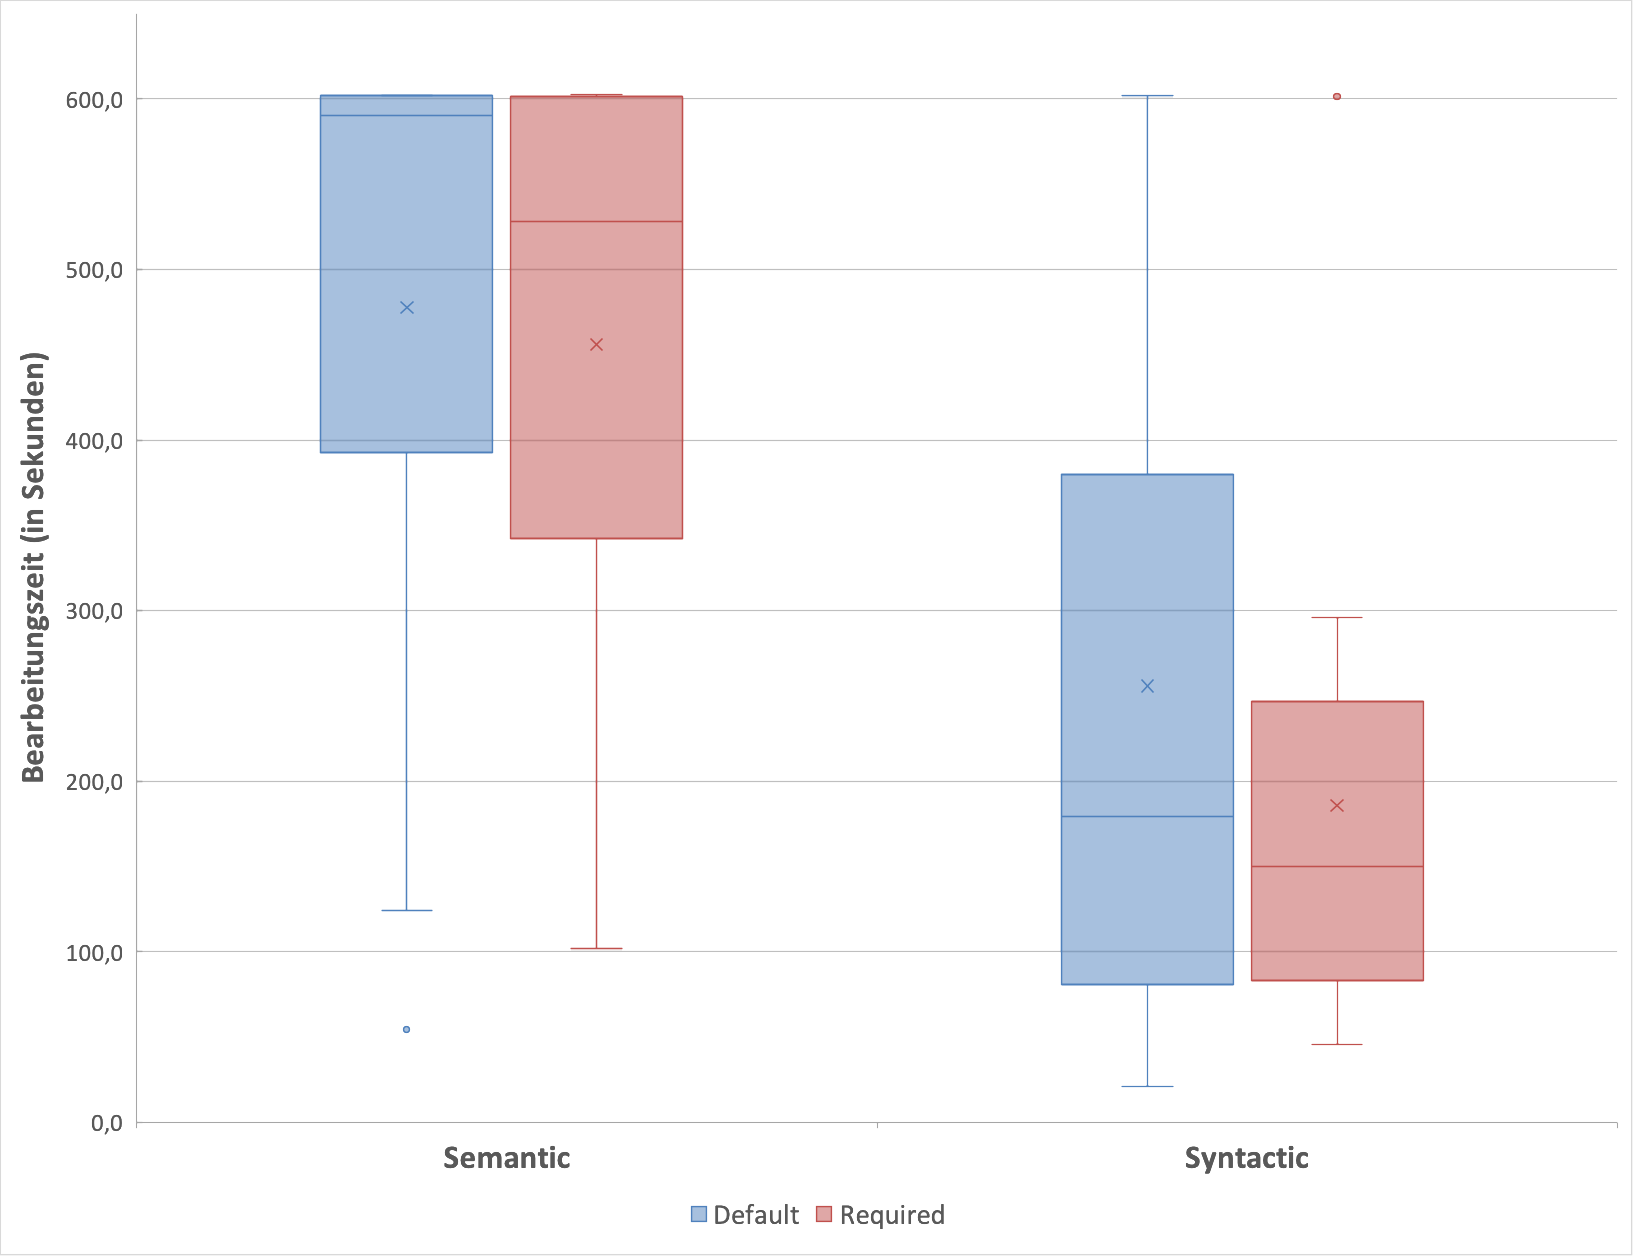
\includegraphics[scale=0.37]{graphics/box_time-constructor.png}
			\caption{\label{fig:box_time-constructor.png} Die Bearbeitungszeit nach Art des Konstruktors}
		\end{figure}
	\end{frame}

	\begin{frame}{Bearbeitungszeit nach AOI}
		\begin{figure}
			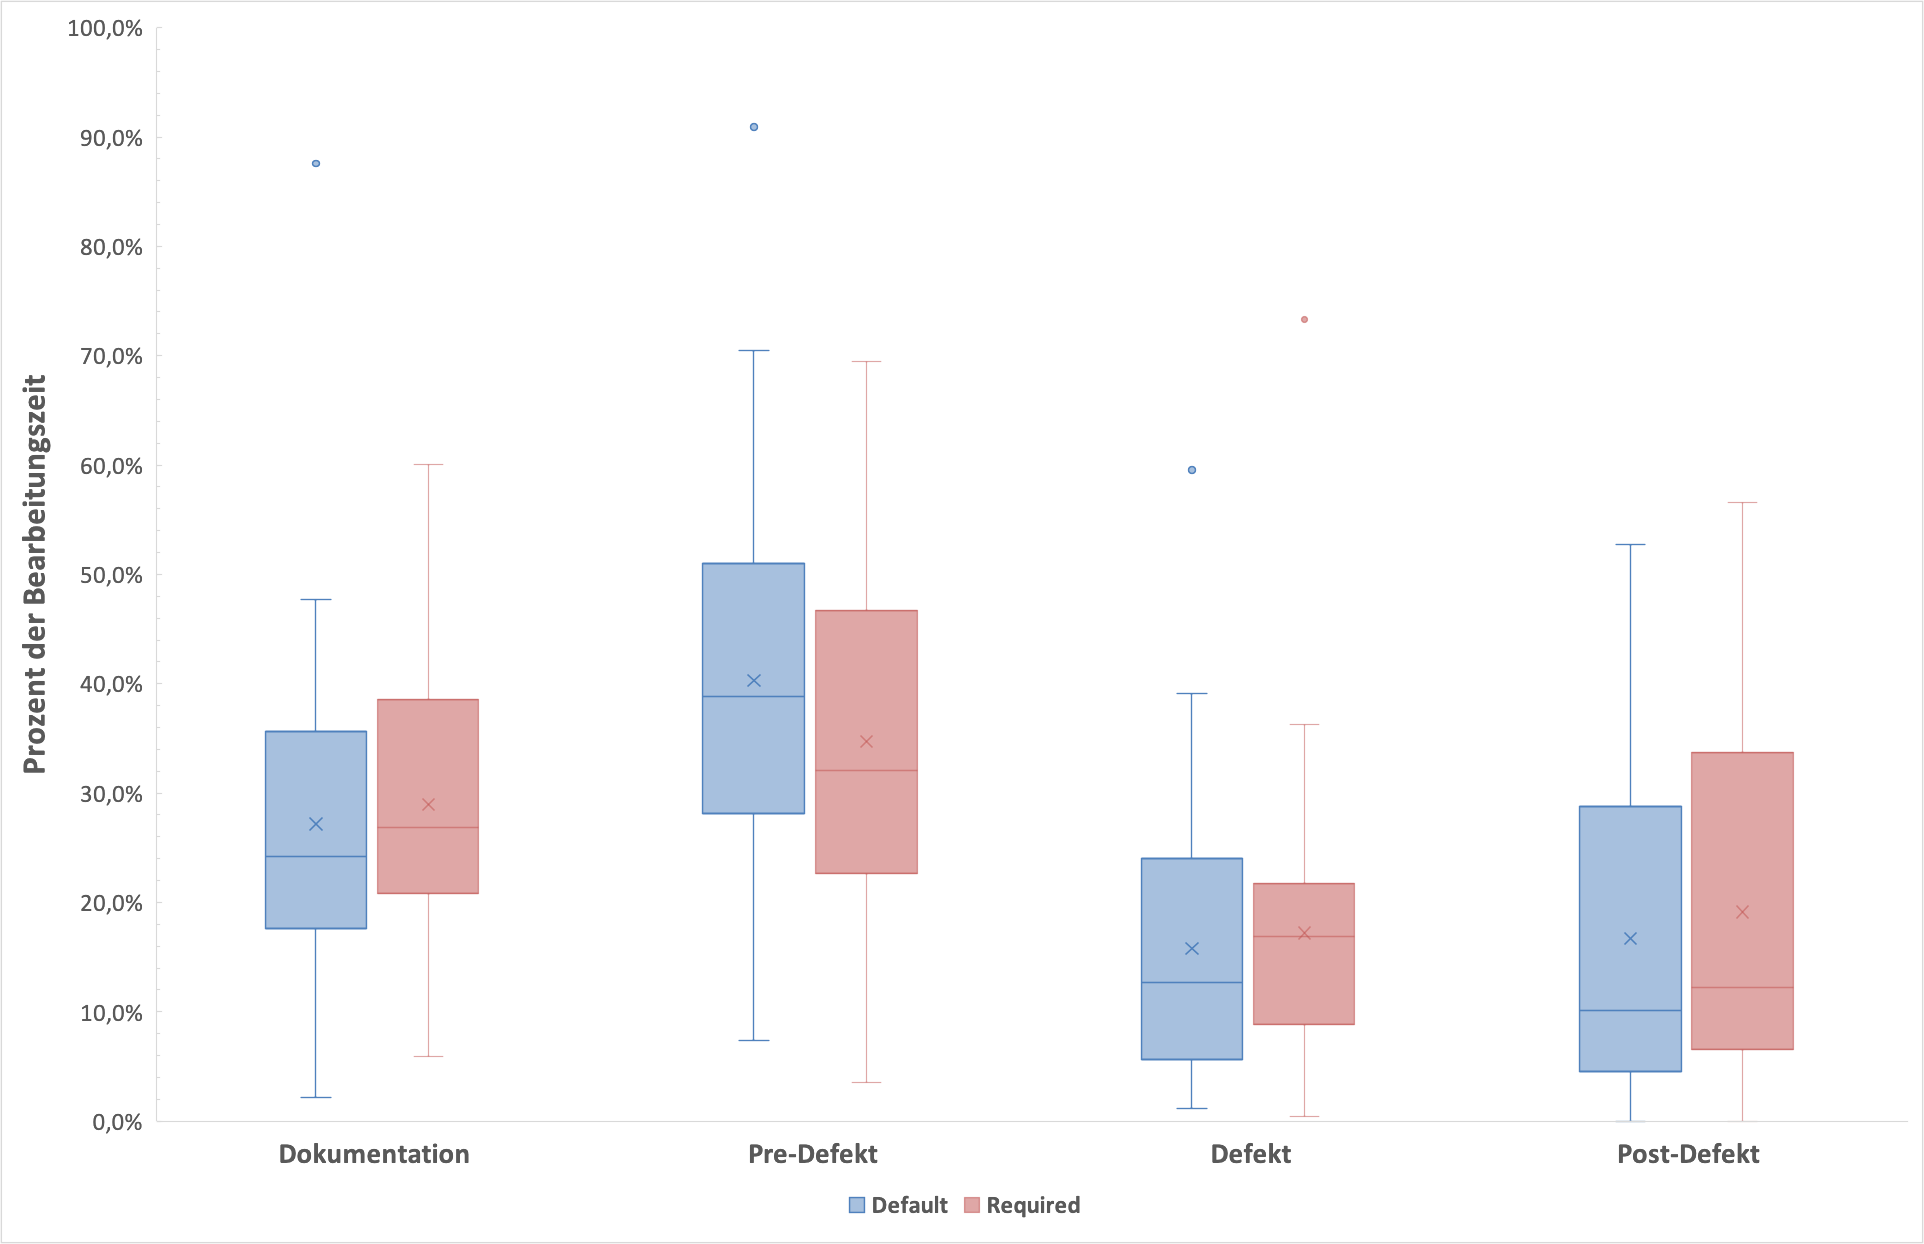
\includegraphics[scale=0.39]{graphics/box_time-aoi_sem.png}
			\caption{\label{fig:box_time-aoi_sem.png} Die Bearbeitungszeit der verschiedenen Areas of Interest (AOI) der semantischen Aufgaben nach Art des Konstruktors}
		\end{figure}
	\end{frame}

	\begin{frame}{Validität}

	\end{frame}	

\section{Vielen Dank für eure Aufmerksamkeit}

\appendix

	\begin{frame}[standout]
		Fragen?
	\end{frame}

%	\begin{frame}[allowframebreaks]{Bibliographie}

%		\bibliography{Presentation}
%		\bibliographystyle{abbrv}

%	\end{frame}

%%% FEATURES %%%

\begin{comment}

	\begin{frame}[fragile]{Typography}
		\begin{verbatim}The theme provides sensible defaults to
		\emph{emphasize} text, \alert{accent} parts
		or show \textbf{bold} results.\end{verbatim}

		\begin{center}becomes\end{center}

		The theme provides sensible defaults to \emph{emphasize} text,
		\alert{accent} parts or show \textbf{bold} results.
	\end{frame}

	\begin{frame}{Font feature test}
		\begin{itemize}
			\item Regular
			\item \textit{Italic}
			\item \textsc{Small Caps}
			\item \textbf{Bold}
			\item \textbf{\textit{Bold Italic}}
			\item \textbf{\textsc{Bold Small Caps}}
			\item \texttt{Monospace}
			\item \texttt{\textit{Monospace Italic}}
			\item \texttt{\textbf{Monospace Bold}}
			\item \texttt{\textbf{\textit{Monospace Bold Italic}}}
		\end{itemize}
	\end{frame}

	\begin{frame}{Lists}
		\begin{columns}[T,onlytextwidth]
			
			\column{0.33\textwidth}
			Items
			\begin{itemize}
				\item Milk \item Eggs \item Potatoes
			\end{itemize}

			\column{0.33\textwidth}
			Enumerations
			\begin{enumerate}
				\item First, \item Second and \item Last.
			\end{enumerate}

			\column{0.33\textwidth}
			Descriptions
			\begin{description}
				\item[PowerPoint] Meeh. \item[Beamer] Yeeeha.
			\end{description}
		\end{columns}
	\end{frame}

	\begin{frame}{Animation}
		\begin{itemize}[<+- | alert@+>]
			\item \alert<4>{This is\only<4>{ really} important}
			\item Now this
			\item And now this
		\end{itemize}
	\end{frame}

	\begin{frame}{Tables}
		\begin{table}
			\caption{Largest cities in the world (source: Wikipedia)}
			\begin{tabular}{@{} lr @{}}
				\toprule
				City & Population\\
				\midrule
				Mexico City & 20,116,842\\
				Shanghai & 19,210,000\\
				Peking & 15,796,450\\
				Istanbul & 14,160,467\\
				\bottomrule
			\end{tabular}
		\end{table}
	\end{frame}

	\begin{frame}{Blocks}
		Three different block environments are pre-defined and may be styled with an
		optional background color.

		\begin{columns}[T,onlytextwidth]
			
			\column{0.5\textwidth}
			\begin{block}{Default}
				Block content.
			\end{block}

			\begin{alertblock}{Alert}
				Block content.
			\end{alertblock}

			\begin{exampleblock}{Example}
				Block content.
			\end{exampleblock}

			\column{0.5\textwidth}
			\metroset{block=fill}
			\begin{block}{Default}
				Block content.
			\end{block}

			\begin{alertblock}{Alert}
				Block content.
			\end{alertblock}

			\begin{exampleblock}{Example}
				Block content.
			\end{exampleblock}

		\end{columns}
	\end{frame}

	\begin{frame}{Quotes}
		\begin{quote}
			Veni, Vidi, Vici
		\end{quote}
	\end{frame}

	\begin{frame}{References}
		Some references to showcase [allowframebreaks] \cite{knuth92,ConcreteMath,Er01,greenwade93}
	\end{frame}

\end{comment}

\end{document}